\section{Lenti}
Tutte le lenti obbediscono alla legge di Snell sulla rifrazione, di conseguenza la geometria della lente determina il modo in cui la luce si propaga attraverso gli elementi ottici. Stabiliremo ora un glossario con la terminologia e introdurremo diverse geometrie di lenti.

\subsection{Terminologia}

\begin{tabularx}{\textwidth}{l p{.8\textwidth}}

D               & 	Diametro – Dimensione fisica della lente.\\
R               &	Raggio di curvatura – La distanza diretta tra il vertice di una superficie e il centro di curvatura.\\
EFL 	        &   Lunghezza focale effettiva – Distanza ottica tra il piano principale di un ottica e il piano immagine.\\
BFL 	        &   Lunghezza focale posteriore – Distanza meccanica tra l'ultima superficie della lente ed il piano immagine.\\
P, P" 	        &   Piano Principale – Piano ipotetico dove i raggi di luce incidenti si piegano a causa del fenomeno della rifrazione.\\
CT              & 	Spessore centrale – la distanza tra il piano principale e la fine dell'elemento.\\
db 	            &   Diametro di ingresso del raggio – Diametro di un raggio collimato in ingresso.\\
dr 	            &    Diametro di uscita del raggio – Diametro di un anello luminoso in uscita all'elemento.\\
L 	            &   Lunghezza distanza effettiva fra le superfici di un elemento.
\end{tabularx}

\subsection{Plano Convex}
Ideale per la collimazione o focalizzazione, utilizzando luce monocromatica.
\begin{figure}[!ht]
\centering

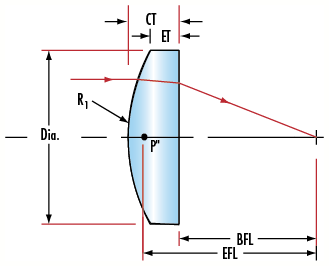
\includegraphics[width=.3\textwidth]{img/plano-convex.png}

\caption{Lente Plano-Convex}
\label{fig:ccd-blockdiagram}
\end{figure}


\subsection{Double Convex}
Ideale per l'inoltro di immagini , e per l'\emph{imaging} di oggetti vicini.
\begin{figure}[!ht]
\centering

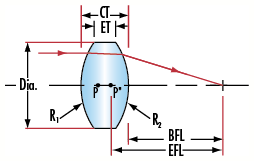
\includegraphics[width=.3\textwidth]{img/double-convex.png}

\caption{Lente Double Convex}
\label{fig:ccd-blockdiagram}
\end{figure}

\subsection{Plano Concave}
Composta da una superficie piatta e una superficie curva verso l'interno. Ideale per l'espansione di fasci, proiezione di luce, ed espansione della lunghezza focale del sistema ottico .

\begin{figure}[!ht]
\centering

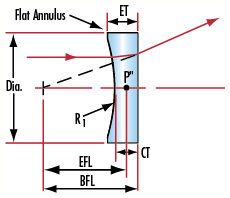
\includegraphics[width=.3\textwidth]{img/plano-concave.png}

\caption{Lente Plano Concave}
\label{fig:ccd-blockdiagram}
\end{figure}


\subsection{Double Concave}
Composto da due superfici equamente curve  verso l'interno. Ideale per l'espansione del fascio, la proiezione di luce e per l'espansione della lunghezza focale del sistema ottico.
\begin{figure}[!ht]
\centering

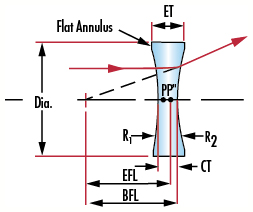
\includegraphics[width=.3\textwidth]{img/double-concave.png}

\caption{Lente Double Concave}
\label{fig:ccd-blockdiagram}
\end{figure}

\subsection{Acromatica positiva}
Esegue funzione simile a quella di una lente PCX o DCX, ma è in grado di fornire dimensioni di punto più piccole e immagini di qualità superiore. Lenti acromatiche sono utili per ridurre l'aberrazione sferica e cromatica
\begin{figure}[!ht]
\centering

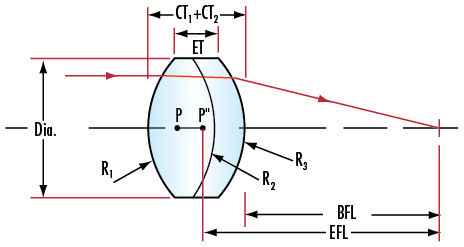
\includegraphics[width=.3\textwidth]{img/positiva-acromatica.png}

\caption{Lente Acromatica positiva}
\label{fig:ccd-blockdiagram}
\end{figure}

\subsection{Asferica}
Ideale per la focalizzazione laser o per la sostituzione di più lenti sferiche in un sistema. Utile per eliminare l'aberrazione sferica  riducendo notevolmente le altre aberrazioni.

\begin{figure}[!ht]
\centering

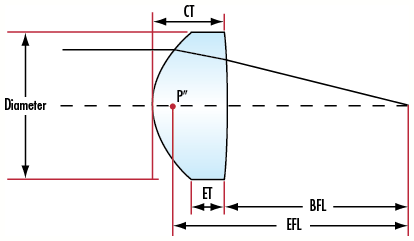
\includegraphics[width=.3\textwidth]{img/asferica.png}

\caption{Lente Asferica}
\label{fig:ccd-blockdiagram}
\end{figure}



